\subsection{Evolutionäre Algorithmen}
Unter evolutionären Algorithmen (EA) verstehen wir randomisierte Heuristiken, die Suchprobleme näherungsweise durch vereinfachende algorithmische Umsetzung von
Prinzipien der natürlichen Evolution zu lösen versuchen. Somit geben evolutionäre Algorithmen in der Regel weder eine Garantie bzgl. der benätigten Rechenzeit noch der Güte der ausgegebenen Lösung. Ein Suchproblem besteht darin, zu einer Zielfunktion ein Element aus deren Definitionsbereich zu finden, dessen Funktionswert möglichst gut ist. Darunter verstehen wir im Folgenden, wenn nicht ausdrücklich anders vermerkt, einen möglichst grossen Funktionswert, weshalb der Zielfunktions wert eines Elements auch als seine Fitness bezeichnet wird.\\

Der Aufbau eines evolutionären Algorithmus lässt sich dann grob wie folgt beschreiben: in jedem Schritt verwaltet er eine Menge fester Grösse von Suchpunkten, die so genannte Population, wobei jeder einzelne Suchpunkt auch als Individuum bezeichnet wird. Aus den Punkten der Population neue Punkte zu erzeugen, ist Aufgabe von Mutation und Rekombination. Dabei steht hinter der Mutation die Idee, jeweils nur ein einzelnes Individuum zufällig zu verändern, ohne dass andere Individuen dabei berücksichtigt werden. Durch Rekombination wird hingegen aus mehreren, meist zwei Individuen zufällig ein neues gebildet, das von diesen möglichst gute Eigenschaften übernehmen soll. Durch Mutation und Rekombination werden also neue Individuen (Kinder genannt) aus bestehenden Individuen (Eltern genannt) erzeugt. Beide Operatoren hängen oftmals stark von Zufallsentscheidungen ab. Jedoch fliesst in der Regel weder in Mutation noch Rekombination der Zielfunktionswert der Individuen ein.\\

Die Zielfunktion beeinflusst nur die Selektion. Dieser Operator wählt Individuen der Population aus, sei es zur Auswahl der Eltern für eine Rekombination oder Mutation oder, um aus der Menge von Eltern und Kindern die nächste Population zu wählen, was den Übergang zur nächsten Generation darstellt. Dadurch, dass die Selektion Punkte mit höherem Zielfunktionswert mit grösserer Wahrscheinlichkeit auswählt, soll erreicht werden, dass nach und nach immer bessere Punkte gefunden werden. \cite{droste}

\begin{figure}[h]
  \centering
  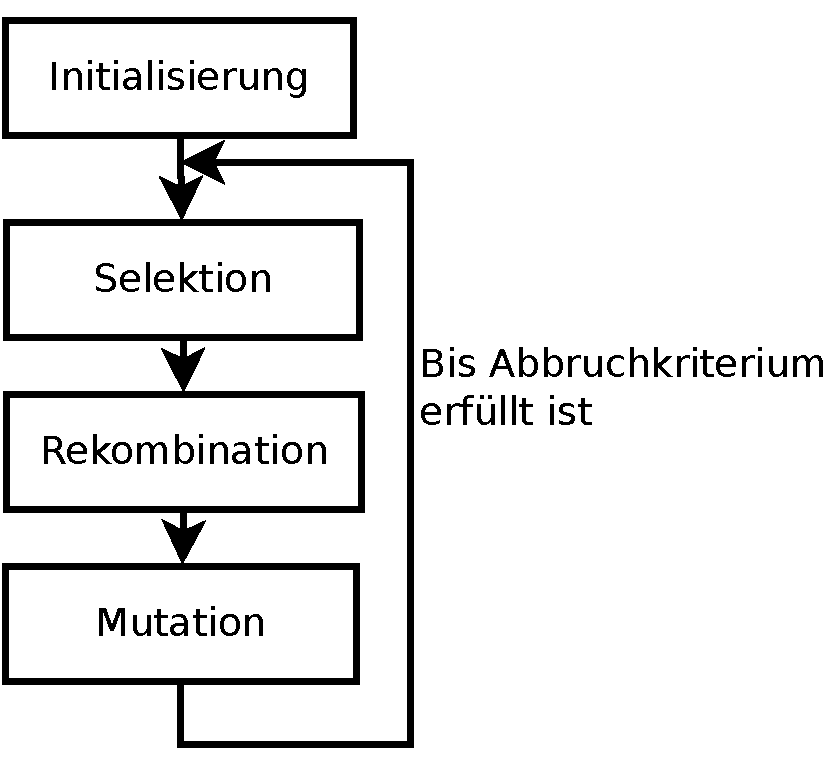
\includegraphics{images/evolutionaerer_algorithmus.pdf}
  \caption[Evolutionärer Algorithmus]{Evolutionärer Algorithmus}
  \label{fig:endlicher_automat}
\end{figure}

\subsubsection{Anwendung auf unser Problem}
TBD